\chapter{Introduction}
\label{introduction}

% \begin{description}
% \item[Problem definition and Significance]: Reverse engineering binary programs can help find software vulnerabilities. Reverse engineering is a hard task that depends on the skill of the reverse engineer. Decompilers exist to help in this process, but their output is still difficult to read and understand. Making reverse engineering easier can help to find vulnerabilities, help researchers quickly understand novel malware, replicate software of which the source code is lost, discover illegitimate usages of intellectual property, porting abandonware, etc. Current approaches mainly focus on recovering aspects lost in the compilation and decompilation process, such as names and types. This fails to address the need for methods to increase the comprehensibility of decompiled code.


% \item[Main Contributions] We propose our code summarisation solution, which takes decompiled functions and synthesises summaries. Our main contributions are a pre-trained, fine-tuned code summarisation model. To create this model we explored the influence of the input types, the impact of data duplication, the impact of different aspects of stripped code and intermediate training on the model performance. We also provide a novel dataset with aligned source code, decompiled code and comments for both stripped and unstripped code.
% \end{description}
% \newpage

\section{Problem Definition and Significance}
Reverse Engineering (RE) is the act of "breaking down" the inner workings of binary executables to analyse and understand programs. It is used to find vulnerabilities and analyse novel malware. Reverse engineering can also help researchers quickly understand novel malware, fingerprint existing malware~\cite{reverseEngineerProcess}, replicate software of which the source code is lost, discover illegitimate usages of intellectual property, porting abandonware, and more~\cite{TypeInferenceSurvey}. The binaries are the most accurate representation of the program that runs on the system, there is no guarantee that the source code represents the binary delivered to the user~\cite{TypeInferenceSurvey}.

Unlike binaries, source code is relatively easy to read, but unfortunately, it is not always available. The original source code is compiled into a runnable binary program by compilers such as Clang/LLVM\footnote{Clang: https://clang.llvm.org/} or GCC~\footnote{GCC: https://gcc.gnu.org/} and delivered to the user. Once compiled, the exact source code version, which was used for compilation, may become unknown or lost altogether.

To understand what a binary program does exactly, the binary code can be decompiled into readable code by decompilers such as Ghidra\footnote{Ghidra Framework: url{https://ghidra-sre.org/}} and IDA Pro.\footnote{IDA Pro: url{https://hex-rays.com/ida-pro/}} Understanding decompiled code is still an intrinsically difficult process. It is a manual, time-consuming process and still largely depends on the skill of the Reverse Engineer~\cite{TypeInferenceSurvey, reverseEngineerProcess}. Much of the work that goes into reverse engineering a binary is spent labelling functions with semantic information~\cite{reverseEngineerProcess}. 

Source code can be described as having two information channels: the algorithmic channel and the natural language channel. The algorithmic channel specifies the execution of a program (semantics), while the natural language channel specifies the purpose and context of the program (syntax)~\cite{dualChannel}. The natural channel includes function and variable names, code comments and the specific human-readable structure of programs. Computers only consider the algorithmic channel to execute a program, while humans use both the algorithmic channel and the natural channel to understand a piece of code~\cite{dualChannel}. Furthermore, code is very regular and predictable, even more so than natural languages~\cite{naturalnessCode}. Language models leverage this naturalness of code~\cite{naturalnessCode} to understand source code.

Due to the naturalness of code, Natural Language Processing (NLP)-based techniques are tailored to the source code as well. For instance, code summarization~\cite{recommend_summarization} is used to automatically generate short natural language descriptions of code. While these methods have been successfully applied to programming languages such as Python, Java and PHP~\cite{CodeT5, CodeBERT, CodeX, PolyglotCodeBERT}, none of these methods has been applied to the relatively syntactically-poor output of decompilers. The compilation process, which transforms readable code into runnable binaries, destroys much of the information contained in the natural channel. Especially stripped binaries - binaries of which the symbol table is removed - will be challenging since they have almost no identifiers at all. Hence, in this thesis we aim to investigate the following goal to address this gap: 
\vskip 1em
\centerline{\textbf{To investigate the application of state-of-the-art code summarisation methods}}
\centerline{\textbf{for decompiled code.}}
\vskip 1em

\section{Contributions}
We, therefore, propose our code summarisation model, which takes decompiled functions and synthesises summaries. Figure~\ref{fig:useCase} shows an overview of the proposed approach. The starting point for a reverse engineer is a binary that a compiler has compiled from source code. This binary is then processed by a reverse engineering tool like Ghidra, which decompiles the binary. From this decompiled code, the functions are then extracted. These decompiled functions are then summarised using our trained CodeT5~\cite{CodeT5} model, which will be discussed in more detail in Chapter~\ref{background}.

\begin{figure}[!tbh]
    \centering
    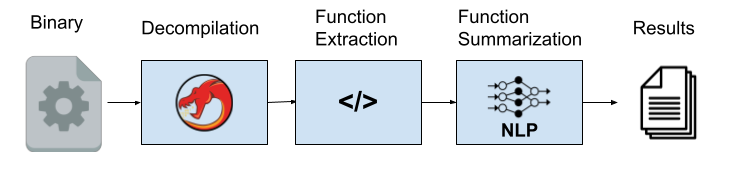
\includegraphics[width=\textwidth,height=\textheight,keepaspectratio]{img/UseCase.png}
    \caption{Proposed solution}
    \label{fig:useCase}
\end{figure}

We perform experiments on this solution to find the impact of decompilation and stripping on the model performance. Furthermore, we investigate the effect of duplicates in the data, and which differences between stripped and unstripped data contribute most to the performance drop. Finally, we use the knowledge from these experiments and design intermediate-training objectives to improve the model's performance on stripped decompiled code.\\

\textbf{Our main contributions can be summarised as follows:}
\begin{description}
 \item[Model:] Our main contribution is a pre-trained, fine-tuned code-summarisation model for decompiled and stripped-decompiled code. The model uses CodeT5 and is fine-tuned and evaluated on our own dataset of source code, decompiled code and stripped-decompiled code pairs. 
 \item[Impact study:] To create this model, we explored the influence of the input types, the impact of data duplication, and the impact of different aspects of stripped and unstripped decompiled code on the model performance.
 \item[Intermediate-training:] To improve the performance of the model, we implemented and evaluated the Neural Machine Translation (NMT), deobfuscation (DOBF) and span-detection (SPAN) intermediate-training objectives. 
 \item[Dataset:] Finally, we contribute the dataset used to fine-tune and pre-train the model. The dataset contains aligned comment-source code, comment-decompiled code, and comment-stripped-decompiled code pairs. We also provide a synthetic dataset of comment-demi-stripped code pairs. Furthermore, we provide the data used for the pre-training objectives. This novel dataset can be used by other works to train and evaluate their models.\footnote{Dataset: \url{https://doi.org/10.4121/20301309}}
\end{description}

\section{Implications}
Several stakeholders can benefit from this research:
\begin{enumerate}
    \item Firstly, security researchers who aim to understand malware. This could help them understand and reverse engineer novel malware more quickly.
    \item Users of closed-source software can use this to inspect the software for faults. Closed source software can be patched, rewritten and reused to serve its exact purposes. Furthermore, understanding the source code can allow users to change the binary in memory during runtime. A malicious example of this group is game hackers who change certain memory addresses to give themselves an unfair advantage (changing their health points, for instance)~\cite{TypeInferenceSurvey}. 
    \item Reverse engineers aim to replicate closed-source software or software of which the source code is lost. Reverse engineering can be used to help create open-source copies or to port the software to newer architectures. Examples range from porting old abandoned open-source projects to porting abandonware (on which copyrights still apply), or even the theft of intellectual property from closed-source commercial software.
    \item On the flip side, creators of closed-source software can use reverse engineering to determine whether other software has copied their products and infringed on their intellectual property.
    \item Lastly, developers of reverse engineering programs and toolkits might be able to use the results of this research to enhance their own products. 
\end{enumerate}

\section{Structure}
The rest of the thesis is outlined as follows: Chapter~\ref{background} will consist of a brief introduction and explanation of concepts and tools used throughout the thesis. In Chapter~\ref{relatedWork} we will discuss other relevant work in this field and how these relate to ours. Chapter~\ref{methodology} will cover the research methodology, the experimental setup will be covered in Chapter~\ref{ExperimentalSetup}. The results will be presented in Chapter~\ref{results}, followed by a discussion on the findings and a short discussion on the threats to validity and ethical considerations in Chapter~\ref{discussion}. Finally, Chapter~\ref{conclusion} will conclude with the findings and discuss possible future works.

